%-----------------------------------------------------------------------------------------------
% 2020-NaaktgeborenC-PolyProc.tex - by C. Naaktgeboren
% License: CC-BY-NC-ND 4.0 - https://creativecommons.org/licenses/by-nc-nd/4.0/
%-----------------------------------------------------------------------------------------------
\documentclass[fleqn,11pt]{SelfArx}
%-----------------------------------------------------------------------------------------------
\usepackage[greek,french,english]{babel}
\usepackage[squaren,cdot]{SIunits}
\usepackage{amsthm}
\usepackage{CormorantGaramond}
%-----------------------------------------------------------------------------------------------
\newcommand{\parxyz}[3]{\left(\frac{\partial {{#1}}}{\partial {{#2}}}\right)_{{#3}}}
\newcommand{\inlxyz}[3]{({\partial {{#1}}}/{\partial {{#2}}})_{{#3}}}
\newcommand{\bri}[2]{(\partial {{#1}})_{{#2}}}
%-----------------------------------------------------------------------------------------------
\newcommand{\GRtxt}[1]{\begin{otherlanguage}{greek}{{#1}}\end{otherlanguage}}
\newcommand{\FRtxt}[1]{\begin{otherlanguage}{french}{{#1}}\end{otherlanguage}}
%-----------------------------------------------------------------------------------------------
\setlength{\abovecaptionskip}{4pt}
\setlength{\columnsep}{5.5mm}
\setlength{\columnseprule}{0.4pt}
\setlength{\fboxrule}{0.4pt} % Width of the border around the abstract
%-----------------------------------------------------------------------------------------------
\definecolor{color1}{RGB}{0,0,90} % Color of the article title and sections
\definecolor{color2}{RGB}{0,20,20} % Color of the boxes behind the abstract and headings
\definecolor{color3}{RGB}{0,0,192} % Color of the article title and sections
%-----------------------------------------------------------------------------------------------
\usepackage[hyperindex,breaklinks]{hyperref} % Required for hyperlinks
\hypersetup{%
    hidelinks,
    colorlinks,
    breaklinks=true,
    urlcolor=color3,
    citecolor=color1,
    linkcolor=color1,
    bookmarksopen=false,
    pdftitle={Title},
    pdfauthor={Author}
}
%-----------------------------------------------------------------------------------------------
\newtheorem{theorem}{Theorem}
\newtheorem{definition}{Definition}
\newtheorem{example}{Example}
\newtheorem{lemma}{Lemma}
\newtheorem{conjecture}{Conjecture}
%-----------------------------------------------------------------------------------------------
\makeatletter
\immediate\write18{datelog > \jobname.info}
\makeatother
%-----------------------------------------------------------------------------------------------
% Journal information
\JournalInfo{Preprints Server Name} % TODO: Update-me
\Archive{Compiled on \input{\jobname.info}}
% Article title
\PaperTitle{On Exact and Locally Polytropic Processes -- Requisites, Etymology, and Modeling}
\Authors{C.~Naaktgeboren\textsuperscript{1$\star$}}
\affiliation{\textsuperscript{1}\textit{Universidade Tecnológica Federal  do  Paraná  --  UTFPR,
Câmpus Guarapuava. Grupo de Pesquisa em Ciências Térmicas.}}
\affiliation{\textsuperscript{$\star$}\textbf{Corresponding  author}:
NaaktgeborenC$\cdot$PhD@gmail$\cdot$com}
\Keywords{Thermodynamics --- Polytropic  Processes  ---  Logical  Processes  ---  Etymology  ---
Modeling}
\newcommand{\keywordname}{Keywords}
\Remarks{%
    defines \emph{logical thermodynamic process} ---
    defines \emph{exact polytropic process} ---
    defines theoretical \emph{requisites} for exact polytropic process ---
    provides \emph{etymology} for the `polytropic' term ---
    presents a novel definition of \emph{locally polytropic process} ---
    proposes  \emph{locally  polytropic  processes}  as  \emph{building  blocks}   for   general
    engineering thermodynamics \emph{process modeling}.
}
\newcommand{\remarkname}{Remarks}
%-----------------------------------------------------------------------------------------------
\Abstract{Work in progress. Here goes the abstract...}
%-----------------------------------------------------------------------------------------------
\begin{document}
%-----------------------------------------------------------------------------------------------

\flushbottom

\maketitle

\tableofcontents

\thispagestyle{empty}

%-----------------------------------------------------------------------------------------------
\section*{License}

    \scriptsize\noindent%
    \begin{minipage}{\columnwidth}
        \centering\tt
        \includegraphics[height=6.0mm]{cc/by-nc-nd.pdf}\\[0.5\smallskipamount]
        {\scriptsize\url{https://creativecommons.org/licenses/by-nc-nd/4.0/}}
    \end{minipage}
    \normalsize

%-----------------------------------------------------------------------------------------------
\section{Introduction}

    Many equilibrium engineering thermodynamics processes  are  taken  to  follow  a  polytropic
    relationship,
    %
    \begin{equation}
        Pv^n = \mathsf{c} = \mbox{const.},
        \label{eq:poly}
    \end{equation}
    %
    \noindent in which $P$ is the system pressure, usually in \kilo\pascal, $v$  is  the  system
    specific volume, usually in $\meter\cubed\!\per\kilogram$,  and  $n$  is  the  dimensionless
    polytropic exponent~\cite{2013-CengelYA+BolesMA-AMGH}---which, for a ``1--2'' process,  with
    initial and final end states labeled as ``1'' and ``2'', can also be written in terms of end
    states properties, as $P_1v_1^n = P_2v_2^n$, which also sets the  particular  value  of  the
    $\mathsf{c}$ constant.

    Some maintream thermodynamics textbooks introduce polytropic processes  in  the  context  of
    closed system boundary work, as a $P\!:\!P(v)$ relationship to plug  in  the  boundary  work
    integral,   which    contains    a    $P\,dv$    integrand~\cite{2013-CengelYA+BolesMA-AMGH,
    2002-MoranMJ+ShapiroHN-LTC, 1985-WylenG-Wiley}. In such texts, the  polytropic  relationship
    is frequently said to find support in measurents, while no specific  theoretical  derivation
    is presented at the point of introduction.

    On  the  other  hand,  other  texts~\cite{1986-JonesJB+HawkinsGA-Wiley,   2006-BejanA-Wiley,
    2015-KroosKA+PotterMC-Cengage} include derivations that lead to a polytropic process, or  at
    least to an isentropic version of it, in which the exponent $n$ has a determined value.

    Moreover, Bejan~\cite[p.~175]{2006-BejanA-Wiley} indicates that a constant  $Pv^n$  relation
    only holds \emph{locally} if the process is such that $n$ is a function of either $P$,  $v$,
    or both.

    A paper due to Christians~\cite{2012-ChristiansJ-IntJMechEngEduc} discusses the topic from a
    perspective  of  teaching  polytropic  processes  themselves,  placing   emphasis   on   the
    \emph{heat-to-work transfer ratio}---named by that author as ``energy transfer ratio''---and
    how its constancy not only yields, but constitutes a  pre-requisite  for  a  process  to  be
    polytropic, besides, naturally, the constancy of the caloric properties of the working  pure
    substance.

    Starting with  an  \emph{etymological}  presentation  of  polytropic  processes,  this  work
    proposes and develops the concepts of \emph{exact polytropic} and \emph{locally  polytropic}
    processes, as well as the supporting concept of \emph{logical thermodynamic} processes,  and
    presents theory-derived \emph{requisites} for a process to be exactly  polytropic.  Finally,
    locally  polytropic  processes  are  proposed  as  discrete  building  blocks  for   general
    engineering thermodynamics \emph{process modeling}.

%-----------------------------------------------------------------------------------------------
\section{Etymology of the `Polytropic' Term}

    The `polytropic' term has its etymology  (origin)  in  the  Greek  language.  This  author's
    sources   on   Greek   are   mostly   based   on   modern   romance   languages,   such   as
    French~\cite{1968-Chantraine-Klincksieck,    2000-BaillyA-Hachette}    and    his     native
    Portuguese~\cite{1997-ManiatoglouMPF-Porto}; therefore, the etymology brought  forth  herein
    will include intermediate French terms.

    The word ``polytropic'' stems from the Greek word  ``\GRtxt{pol'utropoc}''  that  itself  is
    composed of two Greek  words:  (i)~``\GRtxt{pol'uc}''\footnote{The  lexical  form  of  Greek
    adjectives is the nominative, singular, masculine. The nominative,  singular,  \emph{neuter}
    of ``\GRtxt{pol'uc}'' is ``\GRtxt{pol'u}''.}, and (ii)~``\GRtxt{tr'opoc}''.

    The Greek adjective  ``\GRtxt{pol'uc}''  includes  meanings  such  as  \FRtxt{\og  abondant,
    nombreux,   vaste   \fg}~\cite{1968-Chantraine-Klincksieck},   i.e.,   abundant,   numerous,
    vast~\cite{2009-BarrierMA+ViviesC-Auzou,  2011-SilvaASM-WMFMartinsFontes}.  The  Greek  noun
    ``\GRtxt{tr'opoc}''  includes   meanings   such   as   \FRtxt{\og   manière,   façon,   mode
    \fg}~\cite{2000-BaillyA-Hachette},      i.e.,      manner,      way,      fashion,       and
    mode~\cite{2009-BarrierMA+ViviesC-Auzou,  2011-SilvaASM-WMFMartinsFontes}---hence,  meaning:
    numerous forms, or many ways.

    The composed Greek noun ``\GRtxt{pol'utropoc}'' is also  lexical,  and  includes  figurative
    meanings such as \FRtxt{\og souple, habile,  industrieux  \fg}~\cite{2000-BaillyA-Hachette},
    i.e., flexible, adaptive, able, laborious~\cite{2011-SilvaASM-WMFMartinsFontes}; as well  as
    meanings    such    as    \FRtxt{\og    versatilité,     très     divers,     très     varié
    \fg}~\cite{2000-BaillyA-Hachette}, i.e., versatility, very diverse, a  great  variety---thus
    indicating the \emph{wide-range} of processes that it is capable of representing.

    In  fact,  from  a  mathematical  standpoint,  Equation~(\ref{eq:poly}),  there  are  really
    infinitely many allowable (possible) values for the real polytropic exponent $n$ and for the
    $\mathsf{c}$ constant; thence, uncountably many processes departing  from  uncountably  many
    initial states. It is this kind of flexibility that is  encoded  in  the  etymology  of  the
    process name.

%-----------------------------------------------------------------------------------------------
\section{Exact and Locally Polytropic Processes}

    %---------------------------------------------------------------------------------------
    \subsection{Logical Processes}

    In equilibrium engineering thermodynamics, a \emph{process}---more properly  a  quasi-static
    or quasi-equilibrium one---is defined in terms of changes from a certain  equilibrium  state
    of a system to another~\cite{2013-CengelYA+BolesMA-AMGH}, with process \emph{path} being the
    (infinite) sequence of (quasi-)equilibrium states visited by the system during the  process.
    A process can be referred to by its path, with implicit or explicit end states.

    It is worth noting that no constraints are stated for the end states of  a  process  in  its
    definition.  This  allows  for  the  needed  flexibility  in  describing  the   variety   of
    transformations systems and control volumes can undergo in engineering thermodynamics.

    This lack of end state constraints in the definition of a process allows them to be splitted
    into multiple, successive `sub-processes' that still fit the definition  of  a  process,  as
    well as merged multiple successive ones together into `super-processes' that  also  fit  the
    definition of a process. This ability is extremely useful in grouping and splitting  systems
    and control volumes along with their underlying processes---a commom practice in engineering
    thermodynamics.

    Conversely, in order to  make  the  intended  distinction  between  proposed  ``exact''  and
    ``locally'' polytropic processes, additional constraints need to  be  made  to  process  end
    states. Thus, the following defines a  \emph{logical  thermodynamic  process},  which  is  a
    thermodynamic process with constrained end  states.  In  context,  i.e.,  in  thermodynamics
    texts, what's defined next can be simply called a ``logical process'':

    \begin{definition}[logical process]\label{def:logical.proc}
        A logical process is one in which its stated defining conditions, that determines all of
        the allowed interactions or property relations for  the  underlying  system  or  control
        volume, uniformly and continually apply to the  entirety  of  its  path  from---but  not
        earlier than---its initial state until---but not later than---its end state.
    \end{definition}

    Therefore,  for  a  simple  compressible  system---one  admitting   only   work   and   heat
    interactions---either stated heat and work interactions, or system property  specifications,
    or combinations of the two, define possible logical processes.

    Moreover, the stated defining conditions of a logical process can also carry  a  ``logical''
    qualifier, as to make it explicit they're being used in the definition of a logical process,
    as  in  the  ``logical  conditions,''  or  ``defining  logical   conditions''   expressions.
    Furthermore, the conditions themselves can carry the ``logical''  qualifier,  for  the  same
    purpose.

    \begin{example}\label{ex:ideal.Diesel}
        The   well-known   air-standard   ideal   Diesel    power    cycle,    illustrated    on
        Figure~\ref{fig:cycle.Diesel}, with ``intake'' state (of lowest temperature and pressure
        and maximum specific volume) labeled as ``1'', can be divided in  different  ways  using
        only logical processes. One such division is:  (i)~``logical  isentropic  compression'',
        ($\Delta s\!=\!0 \therefore Q\!=\!0$, $W\!\!<\!0$), (ii)~``logical  isobaric  heating'',
        ($Q\!>\!0$,  $\Delta  P\!=\!0   \therefore   W\!\!>\!0$),   (iii)~``logical   isentropic
        expansion'', ($\Delta s\!=\!0  \therefore  Q\!=\!0$,  $W\!\!>\!0$),  and  (iv)~``logical
        isochoric  cooling'',  ($Q\!<\!0$,  $\Delta  v\!=\!0   \therefore   W\!\!=\!0$),   which
        correspond, respectively, to the ``1--2'', ``2--3'', ``3--4'', and  ``4--1''  processes,
        i.e., to the canonical  processes  for  this  cycle,  excluding  sub-processes  thereof.
        Another possible division is: (a)~``logical isentropic compression'',  ($\Delta  s\!=\!0
        \therefore   Q\!=\!0$,   $W\!\!<\!0$),   (b)~``logical   no-heat-removal    expansion'',
        ($Q\!\geqslant\!0$, $W\!\!>\!0$), and  (c)~``logical  isochoric  cooling'',  ($Q\!<\!0$,
        $\Delta v\!=\!0 \therefore W\!\!=\!0$), which correspond, respectively, to the ``1--2'',
        ``2--4'' (through ``3''), and ``4--1'' processes, excluding sub-processes thereof, since
        these encompass the farthermost end states that uniformly and  continually  embrace  the
        stated defining logical conditions (a), (b), and (c).
    \end{example}

    \begin{figure}[ht]
        \centering
        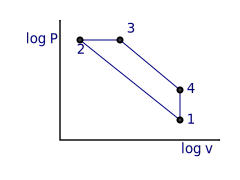
\includegraphics[width=40mm]{fig/idealDieselExample.pdf}
        \caption{Air-standard ideal Diesel cycle in  logarithmic  $P\times  v$  coordinates,  in
            support for the Example~\ref{ex:ideal.Diesel}.}
        \label{fig:cycle.Diesel}
    \end{figure}

    %---------------------------------------------------------------------------------------
    \subsection{Exact Polytropic Processes}

    One is now in a position to define \emph{exact polytropic processes}:

    \begin{definition}[exact polytropic process]\label{def:exact.poly.proc}
        An exact polytropic process is a  logical  process  in  which  either  (i)~a  polytropic
        relation $Pv^n = \mbox{const.}$, with a  unique  polytropic  exponent  $n$,  or  (ii)~an
        isochoric logical condition, can be its sole logical defining condition,  provided  that
        no state in its path is visited more than once or serves simultaneously as  initial  and
        final end states in a given execution.
    \end{definition}

    It is worth noting that isochoric processes are equivalent to polytropic processes  with  $n
    \to \pm\infty$ between stated end states. Definition~\ref{def:exact.poly.proc} accounts  for
    the isochoric process non-unique polytropic exponent by explicitly including it as  a  valid
    exact polytropic process.

    \begin{lemma}\label{lemm:no.reversal}
        Any logical process defined by a single polytropic relation  with  a  unique  polytropic
        exponent, with non-identical end states can only be an exact polytropic process  in  the
        absence of reversals in its path.
    \end{lemma}

    \begin{proof}
        Let a logical process $\mathcal{P}_{1,2}$ be defined by  a  single  polytropic  relation
        with a unique polytropic exponent $n$, with non-identical end states ``$1$'' and ``$2$''
        that contains a set of reversal  states  ``$r_i$'',  with  $\{  i  \in  \mathbb{Z}  |  i
        \geqslant 1 \}$ in its path.

        Without loss of generality, let further $P_{r_1}  <  P_1$,  if  $n  \neq  0$,  i.e.,  an
        initially pressure-decreasing process---since the following argument  can  be  otherwise
        flipped, or laid out in $v$, for finite $n$:

        Let state ``$\epsilon$'', defined as $(P_{\epsilon}, v_{\epsilon})$, belong to the  path
        of   a   sub-process   $\mathcal{P}_{1,r_1}$   of   the   original    logical    process
        $\mathcal{P}_{1,2}$, so that
        %
        \begin{equation}
            P_{\epsilon} - P_{r_1} = \Delta P \to 0.
            \label{eq:proof.Delta.P.epsi}
        \end{equation}
        %
        Since $\mbox{``}\epsilon\mbox{''} \in  \mathcal{P}_{1,r_1}  \in  \mathcal{P}_{1,2}$,  it
        follows from the definition of $\mathcal{P}_{1,2}$:
        %
        \begin{equation}
            P_{\epsilon}v_{\epsilon}^n = P_1v_1^n = P_{r_1}v_{r_1}^n.
            \label{eq:proof.Process.epsi}
        \end{equation}
        %
        Since at ``$r_1$'', the process experiments a reversal, thus proceeding with  increasing
        pressures. Let state ``$\zeta$'', defined as $(P_{\zeta},  v_{\zeta})$,  belong  to  the
        path  of  a  sub-process  $\mathcal{P}_{r_1,2}$  of   the   original   logical   process
        $\mathcal{P}_{1,2}$, so that
        %
        \begin{equation}
            P_{\zeta} \equiv P_{\epsilon} = \lim_{\Delta P \to 0} P_{r_1} + \Delta P,
            \label{eq:proof.P.zeta}
        \end{equation}
        %
        \noindent  so  that  process  $\mathcal{P}_{r_1,2}$  is  guaranteed  to  contain   state
        ``$\zeta$'', since state ``$r_1$'' is a  reversal  one,  rather  than  a  stopping  one,
        therefore:  $\mbox{``}\zeta\mbox{''}  \in  \mathcal{P}_{r_1,2}  \in  \mathcal{P}_{1,2}$,
        implying:
        %
        \begin{align}
            P_{\zeta}v_{\zeta}^n & = P_{r_1}v_{r_1}^n = P_{\epsilon}v_{\epsilon}^n\quad\mbox{(by
            Eq.~(\ref{eq:proof.Process.epsi}))}\quad\rightharpoondown
            \label{eq:proof.Process.zeta} \\
            P_{\epsilon}v_{\zeta}^n & = P_{\epsilon}v_{\epsilon}^n \quad\rightharpoondown \\
            v_{\zeta}^n & = v_{\epsilon}^n \quad\rightharpoondown \\
            v_{\zeta} & = v_{\epsilon}.
            \label{eq:proof.vzeta=vepsi}
        \end{align}
        %
        From  Eqs.~(\ref{eq:proof.P.zeta})  and~(\ref{eq:proof.vzeta=vepsi}),  one  has   states
        ``$\epsilon$''  and  ``$\zeta$''  are  identical:   $\mbox{``}\epsilon\mbox{''}   \equiv
        \mbox{``}\zeta\mbox{''}$, with $\mbox{``}\epsilon\mbox{''}  \in  \mathcal{P}_{1,2}$  and
        $\mbox{``}\zeta\mbox{''} \in \mathcal{P}_{1,2}$.

        Therefore,      by      the       exact       polytropic       process       definition,
        Definition~\ref{def:exact.poly.proc}, logical process $\mathcal{P}_{1,2}$ cannot  be  an
        exact   polytropic   process,   since   there   is   at    least    one    state---state
        ``$\epsilon$''---that is visited more than once in a given execution.
    \end{proof}

    \noindent\textit{Remarks:\/}~given that the polytropic  exponent  is  unique,  any  reversal
    would cause the underlying system or control volume to re-visit states already covered, thus
    violating the exact polytropic process definition.

    \begin{theorem}[Cycle]\label{theo:cycle}
        No cycle is an exact polytropic process.
    \end{theorem}

    \begin{proof}
        The defining feature of a cycle of same end states directly violates the restriction  of
        no same initial and end states.
    \end{proof}

    \noindent\textit{Remarks:\/}~even if a cycle can be collapsed down as  to  be  described  in
    terms of a single polytropic process, such as an ideal Diesel cycle with fuel cut ratio $r_c
    \equiv v_3 / v_2 = 1$, the fact that  such  a  cycle  must  invariably  make  at  least  one
    reversal, as to cycle back to previous states, Lemma~\ref{lemm:no.reversal} would constitute
    a second reason to disqualify the cycle as a (single) exact polytropic process.

    For an exact polytropic process, one has, between its end states extrema:%
    %
    \begin{align}
        Pv^n & = c_1 = \text{const.}        & \rightharpoondown\\
        \log(Pv^n) & = \log(c_1) \equiv c_2 & \rightharpoondown\\
        \log P + n\log v & = c_2            & \rightharpoondown\\
        \log P & = -n\log v + c_2. \label{eq:affine}
    \end{align}
    %
    Equation~(\ref{eq:affine}) is an affine relationship between $\log P$ and $\log v$---a  line
    segment that links the process end states extrema---in which  the  polytropic  exponent  $n$
    figures as the negative of the line segment slope.

    Figure~\ref{fig:cycle.Diesel} is drawn in $\log P \times \log v$  coordinates,  and  depicts
    one line segment between each  adjacent  labeled  state  pairs  ``$1$--$2$'',  ``$2$--$3$'',
    ``$3$--$4$'', and ``$4$--$1$'', in which  all  labeled  states  are  extrema  of  each  line
    segment,  and  there  are  no  reversals.  Therefore,  all  such  processes,  enumerated  on
    Example~\ref{ex:ideal.Diesel} with roman numerals (i)--(iv), are exact polytropic ones.

    %---------------------------------------------------------------------------------------
    \subsection{Locally Polytropic Processes}

    Figure~\ref{fig:non.exact} illustrates a process that plots as a curved segment in  $\log  P
    \times \log v$ coordinates. Basic derivative knowledge allows us to think of such process as
    one with a continuously variable slope in double logarithmic $P\times v$ coordinates, which,
    allied to the concluisions  drawn  from  Equation~(\ref{eq:affine}),  to  a  polytropic-like
    relationship with continuously varying exponent $n$.

    \begin{figure}[ht]
        \centering
        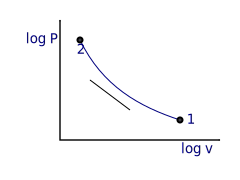
\includegraphics[width=40mm]{fig/nonExactPolytropic.pdf}
        \caption{A process displaying a curve in logarithmic $P\times v$ coordinates.}
        \label{fig:non.exact}
    \end{figure}

    Attempting to \emph{exactly} represent the process as a set of straight line segments  would
    result in an infinite set of segments of vanishing length---hence, with same end states. The
    definition of exact polytropic processes forbids any process in such a set to  be  an  exact
    polytropic one; thus, the following Lemma:

    \begin{lemma}[continuously curved process]\label{lemm:curved.proc}
        A process whose path curve  in  $\log  P  \times  \log  v$  coordinates  displays  in  a
        continuously curved fashion has no exact polytropic sub-process segments.
    \end{lemma}

    If, however, one allows for approximations, as is commom practice in engineering, the curved
    process can be represented by an increasing but  finite  amount  of  line  segments  with  a
    decreasing amounts of deviation (errors). The beginning of such  a  process,  in  which  the
    amount of line segments is doubled at each step, is depicted, with a shift in  $v$  for  the
    sake of improved visualization, on Figure~\ref{fig:approx}.

    \begin{figure}[ht]
        \centering
        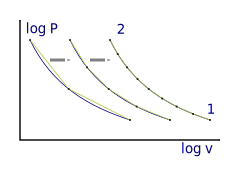
\includegraphics[width=40mm]{fig/approximations.pdf}
        \caption{Successive approximations to the curved process, in dark blue  solid  line,  by
            means of 2, 4, and 8 line segment sub-processes, in  dark  yellow  solid  lines,  in
            double  logarithmic  $P\times  v$   coordinates   (shifted   in   $v$   for   easier
            visualization)}
        \label{fig:approx}
    \end{figure}

    The rationale behind Figure~\ref{fig:approx} is in support of the following definition:

    \begin{definition}[locally polytropic process]\label{def:locally.polytropic}
        A locally polytropic process is one that approximates a  process  in  a  finite  $(P,v)$
        vicinity of it, within suitable error intervals and with at least  one  tangent  or  two
        secant states in common with it.
    \end{definition}

    Regarding envisioned  capabilities  of  locally  polytropic  processes  in  the  context  of
    equilibrium thermodynamics, one herein states:

    \begin{conjecture}[general approximability]\label{conj:gen.approx}
        Any  continuous,  quasi-equilibrium  process  set  of  finite  complexibility   can   be
        approximated within a finite degree of precision by a finite set of  locally  polytropic
        processes.
    \end{conjecture}

    \noindent\textit{Rationale:\/}~it follows from Definition~\ref{def:locally.polytropic}  that
    a finite amount of locally polytropic process  can  approximate,  within  suitable  (finite)
    error intervals, each one  of  the  continuous,  quasi-equilibrium  process  set  of  finite
    complexibility stated on the general approximability conjecture.\vspace{1ex}

    \noindent\textit{Remarks:\/}~it  is  worth  noting  that   all   equilibrium   thermodynamic
    \emph{cycles} of finite complexibility can be subdivided into the process set stated on  the
    general approximability conjecture, above.

%-----------------------------------------------------------------------------------------------
\section{Requisites for Exact Polytropic Processes}

    One can show that the polytropic relation, Equation~(\ref{eq:poly}), is the solution of
    %
    \begin{equation}
        \frac{dP}{P} = -n\frac{dv}{v},
        \label{eq:poly.ODE}
    \end{equation}
    %
    \noindent with $n$ not a function of either $P$ or $v$:
    %
    \begin{align}
        \int\frac{dP}{P} & = -n\int\frac{dv}{v} & \rightharpoondown
        \\
        \log P + \mathsf{c_1} & = -n\log v + \mathsf{c_2} & \rightharpoondown
        \\
        \log P & = -n\log v + \mathsf{c_3} & \rightharpoondown
        \\
        \log P + n\log v & = \mathsf{c_3} & \rightharpoondown
        \\
        Pv^n & = e^{\mathsf{c_3}} \equiv \mathsf{c},
    \end{align}
    %
    \noindent thus recovering Equation~(\ref{eq:poly}).

    The  work  of  Christians~\cite{2012-ChristiansJ-IntJMechEngEduc}  shows   that   internally
    reversible processes in closed systems with a callorically perfect gas with  a  $Pv  =  ZRT$
    equation of state with constant compressibility factor $Z$, defined  as  $Z  \equiv  Pv/RT$,
    assuming negligible changes in system kinetic and potential  energies  and  constant  energy
    transfer ratio,
    %
    \begin{equation}
        K \equiv \frac{\delta q}{\delta w},
        \label{eq:def.K}
    \end{equation}
    %
    \noindent yield a polytropic relation between $P$ and $v$ with a constant exponent $n = (1 -
    \gamma)K + \gamma$.

    In this work, $K$ is also reffered to as \emph{heat-to-work transfer ratio}.

    The employed $Pv = ZRT$ equation of state is indicative of real gases; however, the constant
    $Z$ assumption narrows down the scope of the result. This prompts the  question  of  whether
    this finding is actually only applicable to ideal gases, for which $Z=1$, or  whether  other
    constants work.

    The energy balance equation for a closed system reads, in the intensive  differential  form,
    as
    %
    \begin{equation}
        \delta q - \delta w = du + de_k + de_p,
        \label{eq:1st.law.int.diff.micro.macro}
    \end{equation}
    %
    \noindent where $\delta q$ and $\delta w$ are the differential heat and  work  interactions,
    following the historical thermodynamic sign convention of positive heat  interactions  being
    into the system and positive work interactions being out of the  system,  as  in  an  engine
    application; $u$ is the system specific internal energy, and $e = e_k + e_p$ is  the  system
    specific macroscopic energy, with $e_k$ and $e_p$ being the specific kinetic  and  potential
    energies, respectively. Neglecting the variation of the system macroscopic energy forms,
    simplifies Equation~(\ref{eq:1st.law.int.diff.micro.macro}), giving:
    %
    \begin{align}
        \delta q - \delta w & = du, & \rightharpoondown
        \label{eq:1st.law.int.diff} \\
        (K-1)\delta w & = du,
        \label{eq:1st.law.int.diff.K}
    \end{align}
    %
    \noindent in which Equation~(\ref{eq:def.K}) is used.

    At  this   point,   reference~\cite{2012-ChristiansJ-IntJMechEngEduc}   replaces   $du$   by
    $c_v\,dT$---where $c_v$ and $c_p$ are the constant-volume  and  constant-pressure  substance
    specific heats, respectively---and continues the analysis with a  $Pv  =  ZRT$  equation  of
    state with the assumption of constant $Z$. Shortly after, the $ZR$ term is replaced by $(c_p
    - c_v)$, which recovers an ideal gas result, as $ZR = (c_p - c_v)$ cannot  hold  in  general
    for a real gas, as, for instance, its error approaches infinity in the close vicinity of the
    critical state, even if appoached from the monophase region, due to $c_p \to  +\infty$  with
    all other quantities remaining finite.

    Moreover, a constant $Z$ must be either based on (i)~ideal gas  behavior  or  on  (ii)~small
    process pressure and temperature variations, as experimental  results  associated  with  the
    real gas equation of state are generalized for $Z\!:\!Z(T_r, P_r)$, where  $T_r$  and  $P_r$
    are respectively the reduced  (dimensionless),  critical-state-normalized,  temperature  and
    pressure.

    On the other hand, the  following  theoretically  demonstrates  that  assuming  $u\!:\!u(T)$
    actually implies $Z\!:\!Z(v)$---a useful intermediate result.

    %---------------------------------------------------------------------------------------
    \subsection{Substance Equation of State Yielding $u\!:\!u(T)$}

    For $u\!:\!u(T)$ to hold, one must have:
    %
    \begin{equation}
        \parxyz uiT = 0.
        \label{eq:uT}
    \end{equation}
    %
    \noindent for \emph{any} choice of property $i$ other than $T$.

    Perhaps the easiest way of deriving the outcomes of Eq.~(\ref{eq:uT}) is by rewriting it  in
    terms of Bridgman's relations~\cite{2006-BejanA-Wiley}, which are expressed in  terms  of  a
    peculiar notation. Therefore, rewriting Eq.~(\ref{eq:uT}) in Bridgman's notation yields
    %
    \begin{equation}
        \frac{\bri uT}{\bri iT} \equiv \parxyz uiT = 0 \quad\rightharpoondown\quad \bri uT = 0.
        \label{eq:uT.bri}
    \end{equation}
    %
    It is worth noting than the $\equiv$ sign on Eq.~(\ref{eq:uT.bri}) indicates the  definition
    of the \emph{ratio} between Bridgman's primitives $\bri  uT$  and  $\bri  iT$  in  terms  of
    $\inlxyz uiT$, rather than the other way around.

    Bridgman's relations are tabulated expressions for its \emph{individual primitives} in terms
    of    thermodynamic    properties    that    are    easily    obtainable    from    physical
    measurements~\cite{2006-BejanA-Wiley}, which makes them ingeniously useful.

    Bridgman's  peculiar  notation  allowed  Eq.~(\ref{eq:uT})  to  be  expressed  in  terms  of
    Bridgman's $\bri uT$ primitive only, thus eliminating  the  role  of  Bridgman's  $\bri  iT$
    primitive, \emph{irrespective of the choice of property $i$}. This  greatly  simplifies  the
    analysis of Eq.~(\ref{eq:uT})'s outcomes.

    From reference~\cite{2006-BejanA-Wiley}, one has
    %
    \begin{align}
        \bri uT & = v(\beta T - \kappa P) = 0 & \rightharpoondown \\
        \beta T & = \kappa P,
        \label{eq:bT.kP}
    \end{align}
    %
    \noindent where $\beta$ is the \emph{volumetric coefficient of thermal  expansion},  or  the
    \emph{volume  expansivity}~\cite{2006-BejanA-Wiley},  or  the  \emph{coefficient  of  volume
    expansion}~\cite{1986-JonesJB+HawkinsGA-Wiley},  and  $\kappa$   is   the   \emph{isothermal
    compressibility}~\cite{2006-BejanA-Wiley}, also denoted by some authors as $\kappa_T$, as to
    distinguish         it         from         the         isentropic          compressibility,
    $\kappa_s$~\cite{1986-JonesJB+HawkinsGA-Wiley}.

    Put differently, Eqs.~(\ref{eq:uT})--(\ref{eq:bT.kP}) indicate that any substance for  which
    $\beta T = \kappa P$ will have $u\!:\!u(T)$ only.

    Eq.~(\ref{eq:defs.aux}) brings forth definitions of $\beta$ and $\kappa$:
    %
    \begin{equation}
        \beta  \equiv \frac{1}{v}\parxyz vTP, \quad\mbox{and}\quad
        \kappa \equiv \frac{-1}{v}\parxyz vPT.
        \label{eq:defs.aux}
    \end{equation}
    %
    Plugging  in  Eq.~(\ref{eq:defs.aux})  on  Eq.~(\ref{eq:bT.kP})   and   using   the   cyclic
    relationship,
    %
    \begin{equation}
        -1 = \parxyz ji\ell \parxyz\ell ji \parxyz i\ell j,
        \label{eq:cyclic}
    \end{equation}
    %
    \noindent gives, after some manipulation,
    %
    \begin{align}
        \parxyz TPv & = \frac{T}{P} & \rightharpoondown \\
        \left(\frac{\partial T}{T}\right)_v & =
            \left(\frac{\partial P}{P}\right)_v & \rightharpoondown \\
        T & = \mathsf{f}(v)P,
        \label{eq:uT.TPv}
    \end{align}
    %
    \noindent with $\mathsf{f}(v)$ arising from the partial integrations. Therefore, this result
    expresses a subtance in which $T \propto  P$  at  constant  volume.  Letting  $\mathsf{f}(v)
    \equiv f(v)/R$, yields
    %
    \begin{equation}
        Pf(v) = RT,
        \label{eq:uT.EoS}
    \end{equation}
    %
    \noindent with $f\!:\!f(v)$ being an arbitrary function of $v$ only.  If  this  equation  of
    state  is  represented  as  $Pv  =  ZRT$,  then  $Z  =  v/f(v)$,  as  previously  announced.
    Equation~(\ref{eq:uT.EoS}) is the most general equation of state for a  substance  that  has
    $u\!:\!u(T)$, and consequently $du = c_v\,dT$.

    %---------------------------------------------------------------------------------------
    \subsection{Specific Heats of a $u\!:\!u(T)$ Substance}

    Writing $s\!:\!s(T, v)$ and differentiating, with $du =  T\,ds  -  P\,dv$  and  the  Maxwell
    relation based on the Helmholtz energy, $\inlxyz svT = \inlxyz PTv$, one arrives at
    %
    \begin{equation}
        ds = \frac{c_v}{T}\,dT + \parxyz PTv\,dv.
        \label{eq:ds.Tv}
    \end{equation}
    %
    Writing $s\!:\!s(T, P)$ and differentiating, with $dh =  T\,ds  +  v\,dP$  and  the  Maxwell
    relation based on the Gibbs energy, $\inlxyz sPT = -\inlxyz vTP$, one arrives at
    %
    \begin{equation}
        ds = \frac{c_p}{T}\,dT - \parxyz vTP\,dP.
        \label{eq:ds.TP}
    \end{equation}
    %
    Equating  the  cross  derivatives  from  the  $dT$  and  $dv$  (or  $dP$)  coefficients   on
    Eqs.~(\ref{eq:ds.Tv}) and~(\ref{eq:ds.TP}), yields~\cite{2013-CengelYA+BolesMA-AMGH}:
    %
    \begin{align}
        \parxyz{c_v}vT & = +T\left(\frac{\partial^2P}{\partial T^2}\right)_v,\quad\mbox{and}
        \label{eq:cv.test} \\
        \parxyz{c_P}PT & = -T\left(\frac{\partial^2v}{\partial T^2}\right)_P.
        \label{eq:cp.test}
    \end{align}
    %
    Eqs.~(\ref{eq:cv.test}) and~(\ref{eq:cp.test}) are to be used  in  determining  whether  the
    specific heats of a substance with equation of  state  given  by  Eq.~(\ref{eq:uT.EoS})  are
    functions of.

    Therefore, from Eq.~(\ref{eq:uT.EoS}), one has:

    %---------------------------------------------------------------------------------------
    \subsection{Energy Balance with a $u\!:\!u(T)$ Model}

    Plugging  in  $du  =  c_v\,dT$  on  Eq.~(\ref{eq:1st.law.int.diff.K})  and   differentiating
    Eq.~(\ref{eq:uT.EoS}) will make a $dT$ appear on both equations. Equating  the  common  $dT$
    leads to
    %
    \begin{equation}
        dT = \frac{K-1}{c_v}Pdv = \frac{Pf'(v)dv + f(v)dP}{R},
        \label{eq:dT.1st.law.EoS}
    \end{equation}
    %
    \noindent where $f'(v) = df/dv$.

    The   goal   now   is   to   write   Eq.~(\ref{eq:dT.1st.law.EoS})   in    the    form    of
    Eq.~(\ref{eq:poly.ODE}), with constant $n$, which yields
    %
    \begin{equation}
        \frac{dP}{P} = - [f'(v) + (1 - K)(\gamma - 1)]\frac{dv}{f(v)},
        \label{eq:Pv.ODE}
    \end{equation}
    %
    \noindent which, by inspection, gives the polytropic exponent as
    %
    \begin{equation}
        n \equiv f'(v) + (1 - K)(\gamma - 1).
        \label{eq:n}
    \end{equation}
    %
    The constancy of $n$ depends on the constancy of $f'(v)$, and $(1 - K)(\gamma - 1)$.

    From constant $f'(v) = df/dv = \mathsf{c_1}$, one has
    %
    \begin{equation}
        f(v) = \mathsf{c_1}v + \mathsf{c_2},
        \label{eq:f.form}
    \end{equation}
    %
    \noindent with constant $\mathsf{c_1}$ and $\mathsf{c_2}$.

    From the constant $K$ criterion

%-----------------------------------------------------------------------------------------------
\section*{Acknowledgments}

    This research received no specific grant from any funding agency in the public, private,  or
    not-for-profit sectors.

    To God be the glory!

%-----------------------------------------------------------------------------------------------

\bibliographystyle{plain}
\bibliography{bibfile}

%-----------------------------------------------------------------------------------------------
\end{document}
%-----------------------------------------------------------------------------------------------
